\chapter{Results}
\label{chapt:Results}
In this chapter we present the gathered date from the experiment described in the previous chapter.
We provide the data gathered from the interview with the participants and the result metrics from executing the different scenario's as well as the data from the performance tests.
Given this data we formulate our conclusions as to which model performs better in which cases. 
When there are threats to the validity of the data we will also try and deal with those when presenting the results for the data.
\section{Results metrics case study}
These are the results of the management experiment where we let two users manage the system for access control. 
We have four cases for each scenario that had to be managed:

\begin{itemize}
    \item Case 1: User 1 with the attribute enhanced role based model
    \item Case 2: User 1 with the attribute based model
    \item Case 3: User 2 with the attribute enhanced role based model
    \item Case 4: User 1 with the attribute based model
\end{itemize}
\clearpage
\subsection{Setup time}

\subsubsection{Data}

\begin{table}[h]
    \begin{tabular}{ |{2cm}|p{2.5cm}|p{2.5cm}|p{2.5cm}|p{2.5cm}|  }
        \hline
        \multicolumn{5}{|c|}{Timing of managing scenarios} \\
        \hline
        Scenario & case 1 & case 2 & case 3  &case 4\\
        \hline
        1 & 58 min    & 26 min    & 40 min    & 18 min\\
        2 & 41 min    & 32 min    & 32 min    & 23 min\\
        \hline
    \end{tabular}
    \caption{Table results timing}
\end{table}

\subsubsection{Conclusion}
Looking at the data we could conclude that the setup time for the attribute based model is at all times lower than the setup time for the attribute enhanced role based model.
However looking at the experiment we did we can see some problems that lead to these results, first of all the order in which the tests were executed.
Since we let them do each scenario with the attribute enhanced role based model first this took more time due to the nature of the scenario, this caused habituation towards the scenario leading to better timings with the attribute based model.
Another factor influencing these results came to light during the interview,  the users pointed out that the user interface for the attribute based model allowed them to add policies much faster than they could add permissions.
\\
\\
Another trend we notice is that the advanced user took most advantage on setup time of using the attribute based model over the attribute enhanced role based model.
This is because this user made more use of negative policies in the attribute based model, since this user already knew most of the specifications of the system it was possible to use that knowledge to work more efficiently with the negative policies.
\\
\\
We can see a pattern with the data that has been gathered, which clearly favours the use of the attribute based model for both users with a bigger gain for the more knowledgeable user on the level of the setup time.
However there are certain issues with the experiment that do not allow us to make this a definitive conclusion, another experiment where we keep in mind the habituation to scenarios and use more model appropriate user interfaces should be done to either confirm or refute these results.
\clearpage

\subsection{Number of rules}
\subsubsection{Data}

\begin{table}[h]
    \begin{tabular}{ |{2cm}|p{2.5cm}|p{2.5cm}|p{2.5cm}|p{2.5cm}|  }
        \hline
        \multicolumn{5}{|c|}{Number of rules used in management scenarios} \\
        \hline
        Scenario & case 1 & case 2 & case 3  &case 4\\
        \hline
        1 & 44    & 45    & 45    & 61\\
        2 & 23    & 28    & 26    & 32\\
        \hline
    \end{tabular}
    \caption{Table results number of rules}
\end{table}

\subsubsection{Conclusion}

From the data we see that the attribute enhanced role based model consistently results in less permissions compared to the number of policies in the attribute based model, even if only marginally in some cases.
We can also see that for the more advanced user this difference is smaller than for the inexperienced user, this because having more and better knowledge of the system allowed this user to make better use of the negative policies option provided by the attribute based model.
\\
\\
We also noticed that the advanced user preferred putting many conditions together while the inexperienced user chose for using small conditions that were easy to understand, leading to more policies in the attribute based model.
This led too a big difference because we could reuse permissions from the attribute enhanced role based model, but once a policy was made with a specific role in mind another policy had to be made for every other role even if they had had the same access rights, which is what the inexperienced user did.
\\
\\
Lastly there is also a discrepancy between the scenario's, for the more difficult but shorter scenario (scenario two) we notice that the experienced user also needs more policies in the attribute based model compared to when using the attribute enhanced role based model. 
\\
\\
The pattern here shows that the attribute enhanced role based model consistently performs better, especially for the inexperienced users.
The benefit of using this model for the number of permissions is also clearly seen when working with more complex scenarios.
The model also allows for reuse of permissions with different roles without adapting them, making it easier to work with.

\clearpage


\subsection{Correctness}

\subsubsection{Data}
\begin{table}[ht]
    \begin{tabular}{ |{2cm}|p{2.5cm}|p{2.5cm}|p{2.5cm}|p{2.5cm}|  }
        \hline
        \multicolumn{5}{|c|}{Correctness of management scenarios} \\
        \hline
        Scenario & case 1 & case 2 & case 3  &case 4\\
        \hline
        1 & 2 errors    & 4 errors    & 2 errors    & 3 errors\\
        2 & 6 errors    & 7 errors    & 6 errors    & 7 errors\\
        \hline
    \end{tabular}
    \caption{Table results correctness}
\end{table}


\subsubsection{Conclusion}

We can see that using attribute based model consistently produced more errors than using the attribute enhanced role based model.
Analyzing the type of errors we notice that these are very similar in both models but that the effects of the errors, when using the attribute based model, are greater.
Just making logical errors has the same effect using both models, however making attribute based errors causes the system to give errors, which fails in every case that policy/permission is used.
Since the attribute based model runs all policies for a given object all access attempts to that object fail since they all have to evaluate that policy. 
With the attribute enhanced role based model on the other hand this effect only happens when that permission is assigned to a given role, not giving an error when the other roles want to access the object.
\\
\\
In the case where errors are being made, which should be limited in order for both models to properly fulfill their tasks, the attribute enhanced role based model is the better choice since it limits the area where the error can lead to faults in the system.

\section{Results interview}
In this section we go over the different questions asked to the test users of the system with the different models and give an analysis of the responses they have given.

\subsection{General questions}
The first three questions are introductory questions asking for what the users had done and not looking for an answer to compare both models.
\clearpage
\textbf{\say{Different models have been tested, can you tell us which features you used and were needed to complete the different scenario's? which actions had to be done to complete these scenario's?} }
\\
\\
The users pointed out that they used most features of the models, the inexperienced used did not make use of the negative policies that could be used with the attribute based model.
\\

\textbf{\say{Were you able to complete all requested actions in the scenario, given the available feature set? Which tasks went well?} }
\\
\\
Both users pointed out they could complete all the requested actions with both models, which shows that the feature set provided by the models was sufficient with the given requirements.
There were questions however on if the current models their implementation would suffice for more complicated systems.
\\

\textbf{\say{When using conditions did you prefer adding 1 permission/policy with complex conditions or multiple permissions/policies with simple conditions?} }
\\
\\
The inexperienced user preferred using smaller and less complex conditions on rules (general term for permissions/policies) while using more rules in the system.
This user felt that doing so made the system more maintainable in the future since there was no need to dissect huge conditions once the requirements changed, it is also easier to understand the rules this way.
The more experienced user on the other hand found that using more complex conditions on rules, but having less rules made it more readable.

\subsection{Opinion based questions}
In this section we take a deeper look into the differences between the models.
\\

\textbf{\say{Which model did you prefer using for management in the different scenario's?} }
\\
\\
Both users pointed out that they preferred using the attribute based model for both scenario's but that much of this can be attributed to the user interface. 
We have made a very basic user interface for both models and it became clear that while for the attribute based model this is sufficient, this was not found to be sufficient for the attribute enhanced role based model.
Below are images that show the interface that users had to see the current policies/permissions in the system, the information in these images was all that was provided.

\begin{figure}[h]
    \centering
    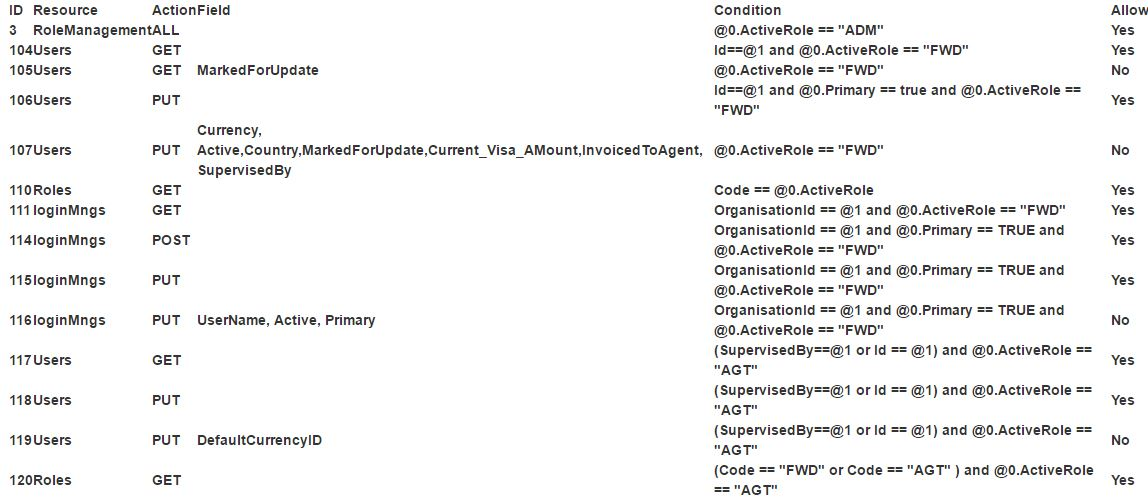
\includegraphics[width=1\textwidth, height=0.24\textwidth]{Img/Tool/ABACPolicies.JPG}
    \caption{Overview policies UI in ABAC}
\end{figure}
\begin{figure}[h]
    \centering
    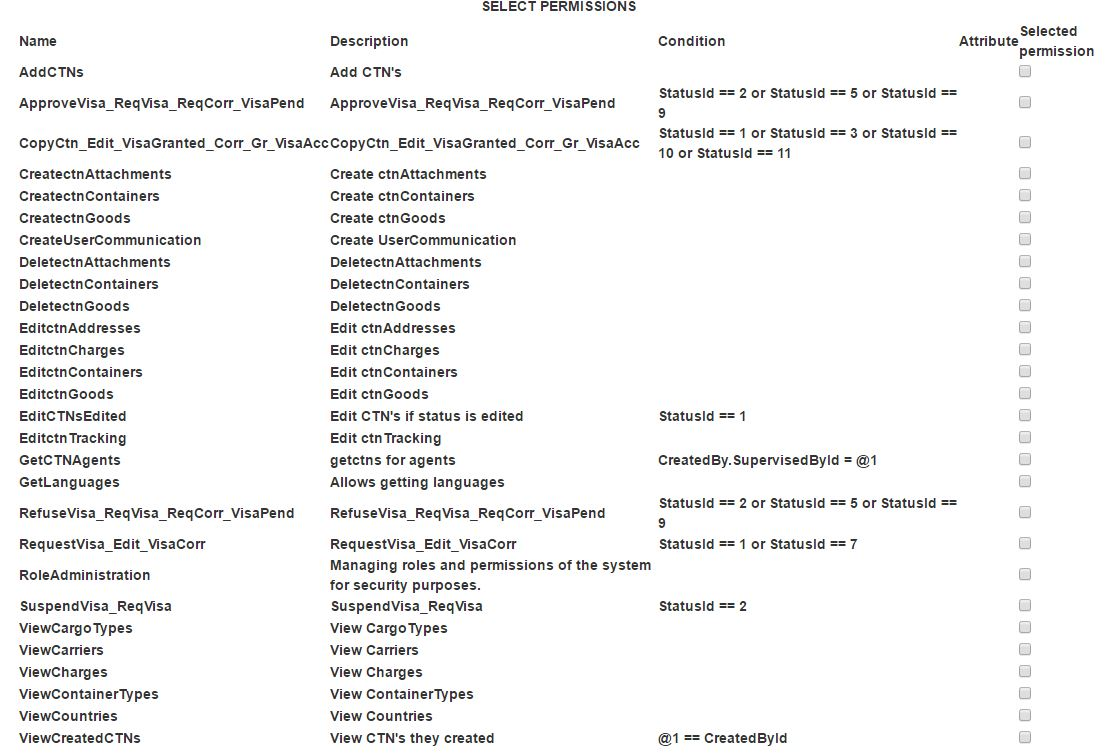
\includegraphics[width=1\textwidth, height=0.24\textwidth]{Img/Tool/RBACPermissions.JPG}
    \caption{Overview permissions UI in AERBAC}
\end{figure}
\\

\textbf{\say{When would you consider the attribute enhanced role based model to be the better choice over the attribute based model? When would you consider using the attribute based model over the attribute enhanced role based model?} }
\\
\\
Users considered the attribute enhanced role based model would perform better than the attribute based model when the system requires the use of many roles, the same was said for systems that have changing requirements, this model was found to be more maintainable.
The attribute based model on the other have was preferred for its quick set up time that the users experienced compared to the attribute enhanced role based model.
It was also preferred when working with systems that do not depend on the use of roles.
\\

\textbf{\say{What is your view on the knowledge that is needed to use the two models effectively? Is there a disparity between the knowledge needed with each model?} }
\\
\\
Both users found that there was no disparity between the two models on the amount of knowledge needed to effectively manage the system.
Both models required a significant amount of knowledge from the user to be used effectively, but since both allow the use of the same type of conditions there is no difference here, apart from conditions being longer with the attribute based model since you need to add in the role check in the conditions.

\textbf{\say{How clear were the interactions between existing policies/permissions and the newly added ones? Was it always clear what the effects of the additions were?} }
\\
\\
The users found that usually it was clear what the effect of adding policies/permissions to the system was, however again due to the interface it was not always clear if the permissions in the attribute enhanced role based system were always assigned correctly to the roles.
One important thing that was pointed out is that you should always keep track of the effects of existing field conditions or adding new ones because these effects can be unclear.
There were however concerns to how this would still be the case when there were many more permissions and policies, but this can be dealt with using filtering.
\\

\textbf{\say{What do you think about the options that are available for constructing conditions?  Would they suffice for the systems you develop? If not what additions could be made?} }
\\
\\
Both users found that the options for making conditions for both systems were sufficient, however it was noted that it would be useful to add negative permissions to the attribute enhanced role based model.
\\

\textbf{\say{Looking at the permissions and policies, how easy to understand is it if you were put there as a new administrator for the system?} }
\\
\\
In its current state it is agreed on that the attribute based model would be clearer for the new admin since that interface contains all the information.
For both models it is also pointed out that the new admin would need significant knowledge of the underlying system, understanding how conditions are made also requires some programming knowledge from the admins and is not fit to be done by non technical personnel.
Using a declarative input language such as XACML\footnote{http://docs.oasis-open.org/xacml/3.0/xacml-3.0-core-spec-os-en.html} would make it more understandable for non technical users.
\\

\textbf{\say{Do you foresee any problems that can arise from using these models in systems that are bigger?} }
\\
\\
The main problems that were foreseen when using the models with a bigger system is that especially with the attribute based model this can gravely impact performance in a negative way.
Concerns were also raised for keeping the oversight of the system but this would not be a big issue for the manageability if we introduce filters and ordering.

\textbf{\say{Are there any features that you think would benefit the different models? What benefits do they provide? Example of possible features: role hierarchy.} }
\\
\\
One user proposed the introduction of negative permissions in the attribute enhanced role based access control model.
We also made a proposal ourselves of adding hierarchical roles to the attribute enhanced role based model, such as discussed in the second chapter.
The users found this to be a good feature to speed up using the model in question, for the attribute based model this extension is not so straight forward since there is no link between roles and policies outside of the conditions.
\\

\textbf{\say{Looking at it as a developer, which model would be best to make the users easily understand their access rights? Why do you think this is the case?} }
\\
\\
The attribute enhanced role based model was considered to be the easiest to develop a visualization for that made it clear for users of the system which rights they had.
This can be attributed to the permissions being linked to the roles, we would not have to make a full evaluation of all the policies available in the system for that object, which would have to be done for the attribute based model.

\subsection{Overall conclusion}
In first instance looking at the results it becomes clear the users generally preferred the attribute based model. 
A lot of that preference had to do with the user interface and how this was setup as has been pointed out by the users.
When looking deeper into this we conclude that if more time is put into a better user interface this will greatly improve the manageability of the attribute enhanced role based model, for the attribute based model there is little improvement to be had using more than the basic interface.
When we only have this basic interface the attribute based model is considered to be the better model on the level of manageability, when we create a more expansive user interface the attribute enhanced role based model will be more manageable. 
\\
\\
On the level of extensibility and understandability the preference goes out to the attribute enhanced role based model.
The link with the permissions and roles makes it easier to visualize to users of the system what they are allowed to do.
This model is also the most extensible model of the two, allowing for easier adaptation.
For maintainability the attribute enhanced role based model was also the one preferred since it did not require many changes to permissions if a new role is added to the system or the requirements change.

\section{Results performance}

\subsubsection{Data}
This data is the average of 100 calls to the system under each of the models, we have the baseline model which is the existing implementation, the attribute enhanced role based model (AERBAC) and the attribute based model (ABAC).
We accessed the system with 3 different users FWD, AGT and ADM.
We have provided the full raw data represented in charts in below, except for the baseline.

\begin{table}[ht]
    \begin{tabular}{ |p{3cm}|p{3cm}|p{3cm}|p{3cm}|  }
        \hline
        \multicolumn{4}{|c|}{Average response time performance} \\
        \hline
        Model & FWD & AGT & ADM\\
        \hline
        Baseline & 0.135 sec   & 0.110 sec   & 0.101 sec  \\
        AERBAC & 0.268 sec    & 9.508 sec    & 0.088 sec  \\
        ABAC & 28.394 sec   & 9.923 sec    & 8.189 sec    \\
        \hline
    \end{tabular}
    \caption{Table results performance}
\end{table}

\begin{figure}[h]
    \centering
    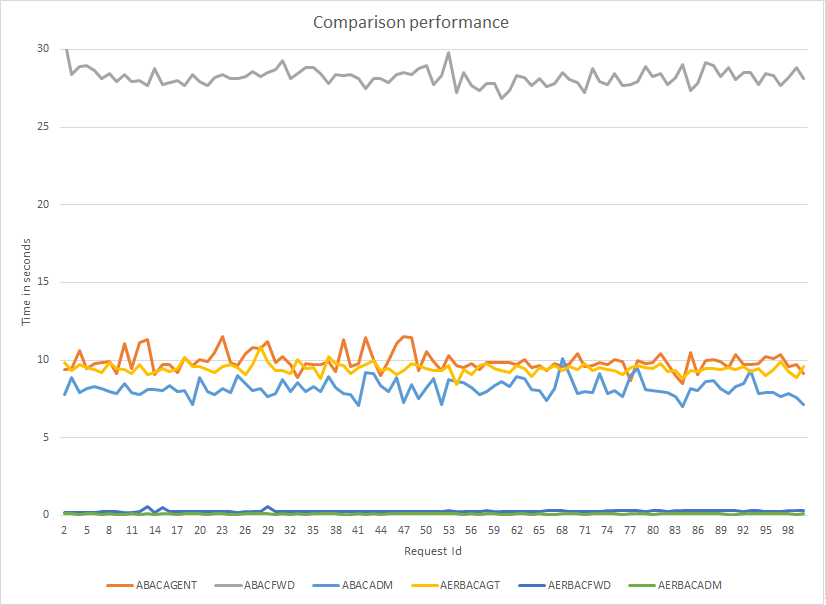
\includegraphics[width=0.9\textwidth, height=0.6\textwidth]{Img/Performance/Perf.png}
    \caption{Comparison implemented models normal scale}
\end{figure}
\begin{figure}[h]
    \centering
    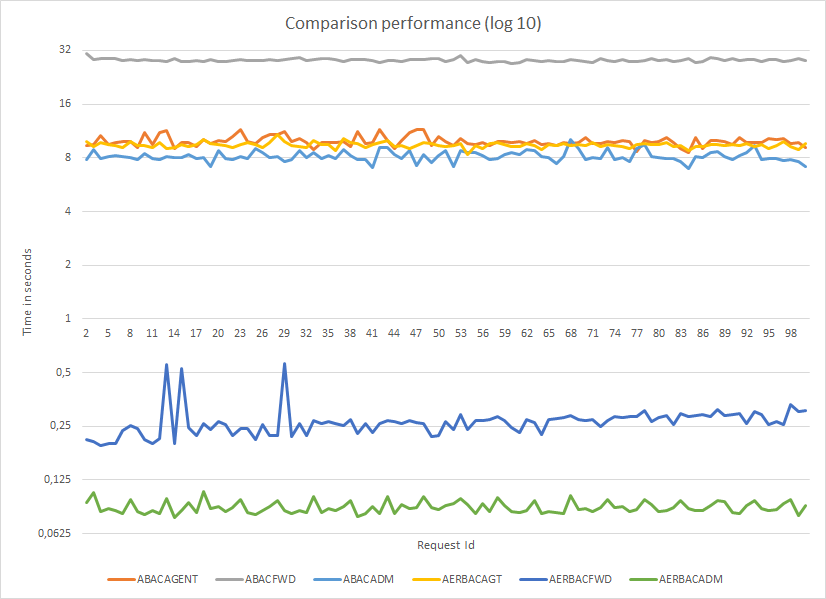
\includegraphics[width=0.9\textwidth, height=0.6\textwidth]{Img/Performance/PerfLog10.png}
    \caption{Comparison implemented models logarithmic scale}
\end{figure}

\subsubsection{Conclusion}
When analyzing this data it becomes clear rather quickly that there are some issues here.
We can see that with the attribute enhanced role based model we still have a performance within the order of magnitude of the base line, in case of the ADM role even better.
However for the agent role we immediately see a performance that is a lot worse.
This issue becomes even more dramatic when we look at the attribute based model.
\\
\\
After searching for where the problem lies it becomes clear that dynamic linq is not mature enough to cope with more complex conditions.
When using conditions that require joins, such as is needed for the AGT role, it does not translate everything to queries which leads to loading all the data in memory.
Further analysis and reasoning between the models can still be done but we need to keep in mind this problem on the implementation level.
\\
\\
One of the first things we notice is that for the attribute enhanced role based model neither the ADM and FWD roles are impacted by this problem.
The reason for this is that the conditions placed are very minimal for both of these roles, they are simple non-combined conditions that do not require any joining of tables.
Looking at these we can also see that the ADM role is still significantly faster than the FWD role.
This is to be attributed to the ADM role having fewer permissions that are assigned to it, while the FWD role has more permissions that are assigned to it for the objects being requested.
This lets us conclude that there is a meaningful impact of the evaluation of the number of permissions assigned to roles on the performance of the models.
This also lets us conclude that the impact on the performance compared to the baseline can be limited and does not pose an issue on the tested scale, given that the problem of the evaluation component can be mitigated.
\\
\\
A second observation is that when using the attribute based model all roles are affected by the problem in the evaluation component.
This while the ADM role especially does not have more conditions or more difficult conditions than with the attribute enhanced role based model.
We see that is is also affected by the problems that manifest themselves with the policies aimed at the AGT role, this is due to the nature the attribute based model works.
Out of this we can conclude that the attribute based model will be slower since it has to evaluate every policy on the object type for every role.
Even if that policy says it is for a different role and lazy evaluation is used, where  we stop evaluating conditions when the result cannot change by any conditions that follow in combination with and/or operators, we still have to do the joins to start evaluating.
Another result is that contrary to the attribute enhanced role based model the FWD role has an even more dramatic performance than the AGT role.
This can be explained due to the complexity of the conditions that  increased using this model.
When actually evaluating the roles lazy evaluation leads to stopping the evaluation of the condition once the first part returns false (comparing the roles).
This prevented more complex and longer condition of being executed for the other roles, but this still impacted the FWD role for which they were meant heavily.
\\
\\
There is one big conclusion that can be made on the level of performance, even with the issues there exists with the evaluation component.
The conclusions being that with the attribute based model we need to evaluate a lot more conditions, with the attribute enhanced role based model on the other hand we first have get the role and extract the permissions assigned to this role and then evaluate the conditions for that role only.
The evaluation of conditions is the more performance intensive operation of the two, which leads to a preference for the attribute enhanced role based model on the level of performance.
However making more conclusions with the current implementation are hard  and difficult to justify.
